(https://www.overleaf.com/5862476167rjmdxcnnhgcg#d5b78c)

\documentclass[12pt,a4paper]{article}

% Paquetes básicos
\usepackage[utf8]{inputenc}
\usepackage[spanish]{babel}
\usepackage{graphicx}
\usepackage{amsmath}
\usepackage{hyperref}
\usepackage{float}
\usepackage{subcaption}
\usepackage{listings}
\usepackage{xcolor}
\usepackage{geometry}
\usepackage{booktabs}

% Configuración de márgenes
\geometry{
    left=2.5cm,
    right=2.5cm,
    top=2.5cm,
    bottom=2.5cm
}

% Configuración de código
\lstset{
    language=Python,
    basicstyle=\ttfamily\small,
    keywordstyle=\color{blue},
    commentstyle=\color{gray},
    stringstyle=\color{red},
    numbers=left,
    numberstyle=\tiny\color{gray},
    breaklines=true,
    frame=single,
    captionpos=b
}

% Información del documento
\title{\textbf{Práctica 01: Aprendizaje por Refuerzo}}
\author{
    Chipichanti -
    \texttt{pablo.chantada@udc.es}\\
    Lauriña -
    \texttt{nome.lo.se@udc.es}\\
    Robótica e Inteligencia Artificial\\
    Universidad de A Coruña
}
\date{\today}

\begin{document}

\maketitle


\section{Introducción}

El aprendizaje por refuerzo (RL) ha demostrado ser efectivo en tareas de control robótico donde el agente debe aprender comportamientos complejos mediante interacción con el entorno. En esta práctica se aborda el problema de seguimiento de objetivo móvil utilizando el robot Robobo en simulación.

\section{Definición del Problema}

\subsection{Espacio de Observaciones}

El espacio de observaciones es \textbf{continuo} (8 dimensiones) y contiene:

\begin{table}[H]
\centering
\begin{tabular}{@{}lll@{}}
\toprule
\textbf{Variable} & \textbf{Rango} & \textbf{Descripción} \\ \midrule
Posición agente (x, z) & [-1, 1] & Posición normalizada del robot \\
Posición objetivo (x, z) & [-1, 1] & Posición normalizada del cilindro \\
Blob visible & \{0, 1\} & Visibilidad del cilindro en cámara \\
Posición blob (x, y) & [-1, 1] & Posición del blob en imagen \\
Tamaño blob & [0, 1] & Tamaño del blob (distancia) \\ \bottomrule
\end{tabular}
\caption{Componentes del espacio de observaciones}
\end{table}

\textbf{Justificación:} Se utiliza espacio continuo para mayor precisión y se combinan datos de posicionamiento absoluto con información visual, permitiendo al agente desarrollar estrategias más robustas.

\subsection{Espacio de Acciones}

El espacio de acciones es \textbf{continuo} (2 dimensiones):

\begin{equation}
\mathbf{a} = [v_{\text{izq}}, v_{\text{der}}] \in [-1, 1]^2
\end{equation}

Donde $v_{\text{izq}}$ y $v_{\text{der}}$ son las velocidades normalizadas de las ruedas izquierda y derecha, que se escalan a velocidades del motor en el rango [-20, 20].

\textbf{Justificación:} Las acciones continuas permiten movimientos más suaves y precisos que acciones discretas, facilitando el seguimiento del objetivo móvil.

\subsection{Función de Recompensa}

La función de recompensa combina múltiples componentes:

\begin{equation}
R_t = R_{\text{dist}} + R_{\text{vis}} + R_{\text{goal}} + P_{\text{dist}}
\end{equation}

Donde:

\begin{itemize}
    \item \textbf{Recompensa por distancia} ($R_{\text{dist}}$):
    \begin{equation}
    R_{\text{dist}} = 0.01 \times (d_{t-1} - d_t)
    \end{equation}
    Incentiva reducir la distancia al objetivo.
    
    \item \textbf{Recompensa por visibilidad} ($R_{\text{vis}}$):
    \begin{align}
    R_{\text{vis}} = \begin{cases}
    0.1 + 0.2 \times (1 - \frac{|x_{\text{blob}} - 50|}{50}) + 0.1 \times \frac{s_{\text{blob}}}{400} & \text{si visible} \\
    -0.3 & \text{si no visible}
    \end{cases}
    \end{align}
    Recompensa mantener el blob visible y centrado.
    
    \item \textbf{Recompensa por objetivo alcanzado} ($R_{\text{goal}}$):
    \begin{equation}
    R_{\text{goal}} = \begin{cases}
    5.0 & \text{si } d_t < 150 \\
    0 & \text{en otro caso}
    \end{cases}
    \end{equation}
\end{itemize}

\textbf{Justificación:} Esta estructura multi-componente guía al agente hacia comportamientos deseados: acercarse (distancia), mantener visión (visual) y alcanzar el objetivo (terminal).

\section{Implementación}

\subsection{Algoritmo de Aprendizaje: SAC}

Se seleccionó \textbf{Soft Actor-Critic (SAC)} por sus ventajas en espacios de acción continuos:

\begin{itemize}
    \item \textbf{Off-policy}: Mayor eficiencia en el uso de datos
    \item \textbf{Maximum entropy}: Fomenta exploración
    \item \textbf{Estabilidad}: Actor-Critic con dos Q-networks
\end{itemize}

\subsection{Hiperparámetros}

\begin{table}[H]
\centering
\begin{tabular}{@{}ll@{}}
\toprule
\textbf{Parámetro} & \textbf{Valor} \\ \midrule
Algoritmo & SAC \\
Learning rate & 3e-4 \\
Gamma (factor de descuento) & 0.99 \\
Batch size & 64 \\
Tau (soft update) & 0.005 \\
Entropy coefficient & auto \\
Train frequency & 1 \\
Gradient steps & 1 \\
Episodios de entrenamiento & 4 \\
Pasos por episodio & 100 \\
\textbf{Total timesteps} & \textbf{400} \\ \bottomrule
\end{tabular}
\caption{Configuración de hiperparámetros}
\end{table}

\subsection{Arquitectura del Sistema}

El sistema consta de tres componentes principales:

\begin{enumerate}
    \item \textbf{Environment} (\texttt{env.py}): Implementa \texttt{gym.Env}
    \item \textbf{Training} (\texttt{train.py}): Entrenamiento con callbacks
    \item \textbf{Evaluation} (\texttt{eval.py}): Validación del modelo
\end{enumerate}

\subsection{Características Especiales}

\textbf{Objetivo Móvil:} El cilindro se mueve cada 5 pasos en direcciones aleatorias ($\pm 20$ unidades), incrementando la dificultad de la tarea.

\textbf{Normalización:} Todas las observaciones están normalizadas en rangos [-1, 1] o [0, 1] para facilitar el aprendizaje.

\section{Resultados Experimentales}

\subsection{Métricas de Entrenamiento}

\begin{figure}[H]
    \centering
    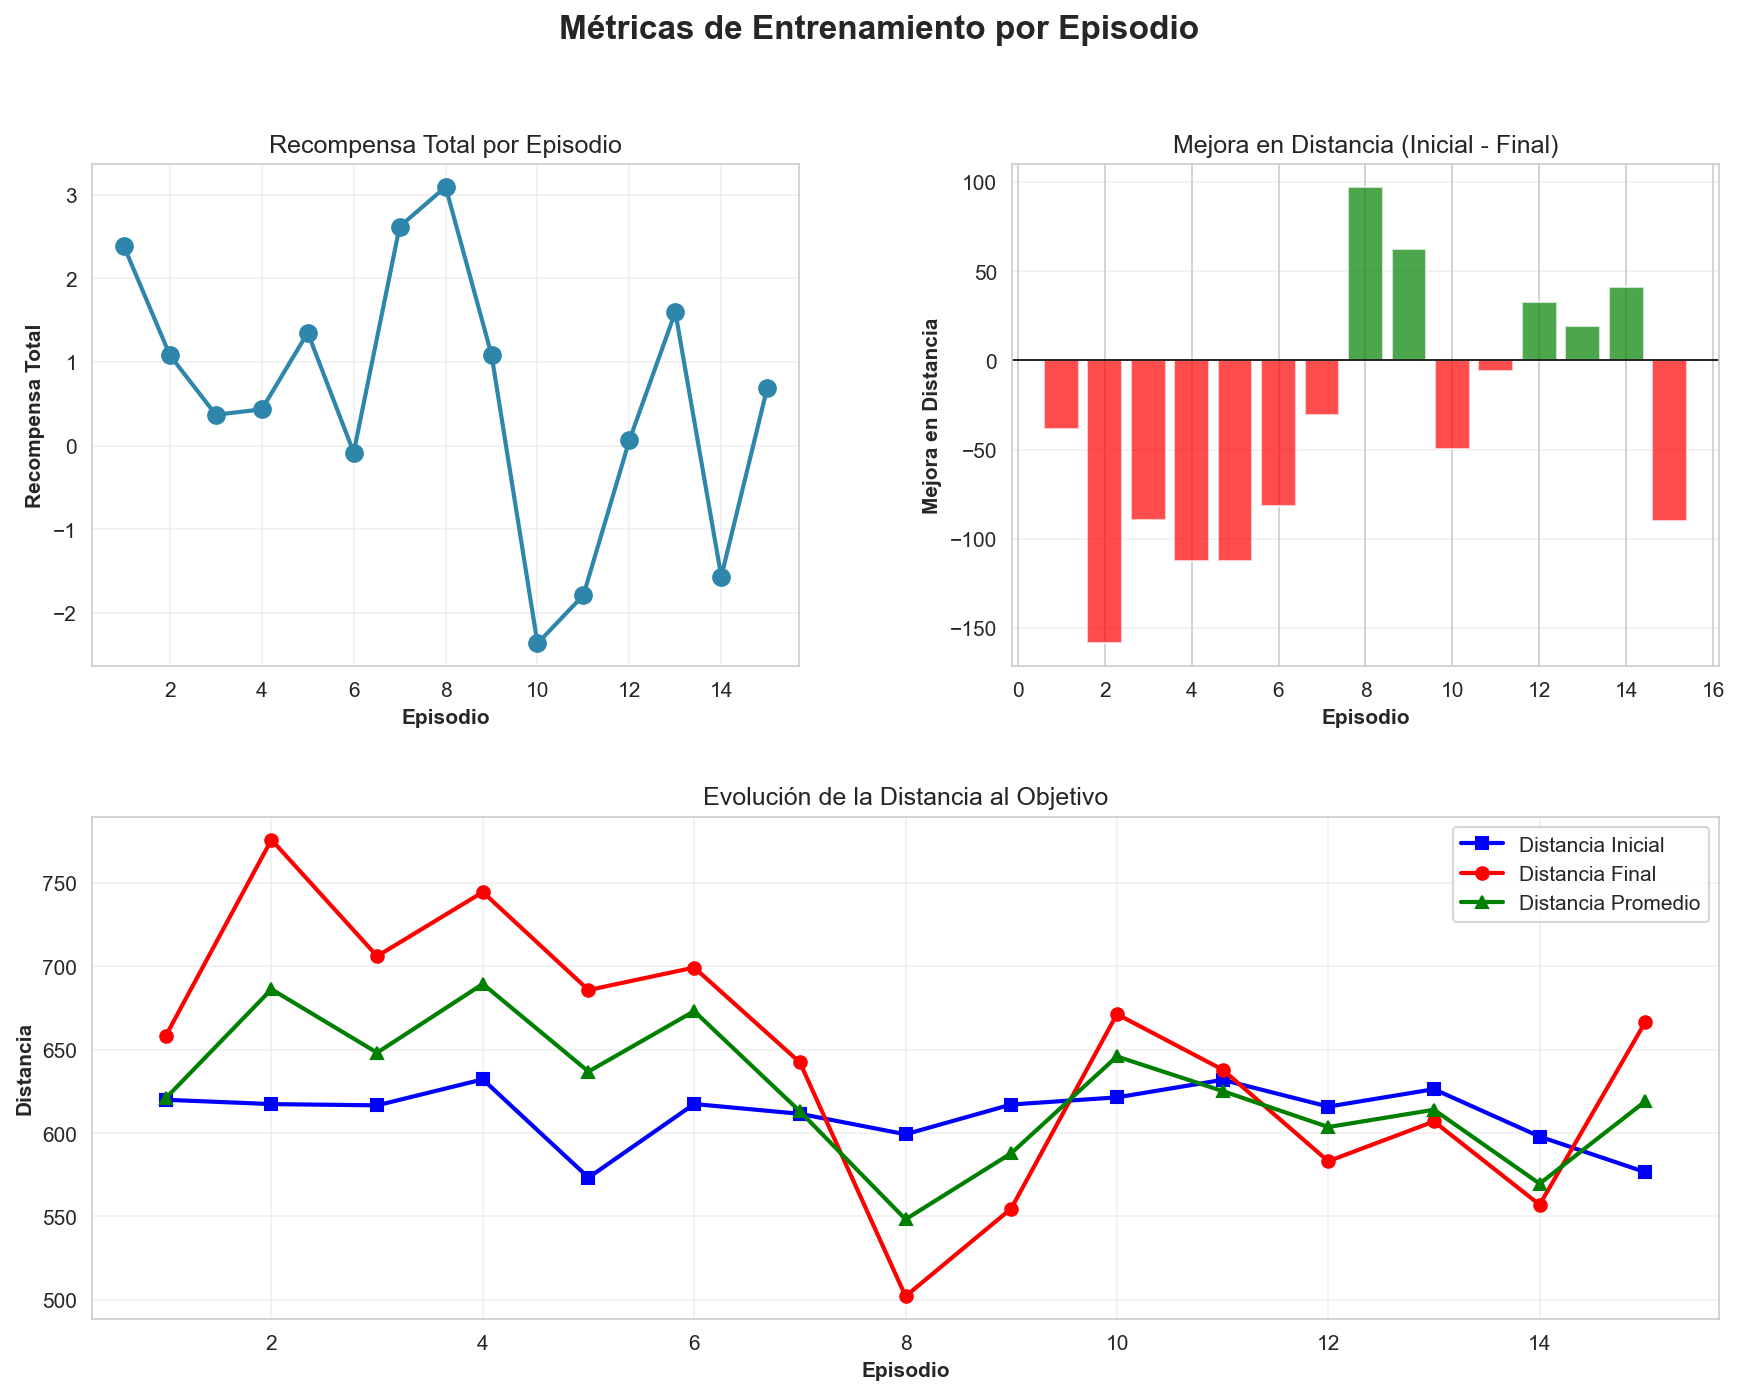
\includegraphics[width=0.9\textwidth]{episode_metrics.png}
    \caption{Evolución de métricas durante el entrenamiento. (a) Recompensa total por episodio. (b) Evolución de distancias. (c) Mejora en distancia respecto al inicio.}
    \label{fig:training_metrics}
\end{figure}

\textbf{Análisis:}
\begin{itemize}
    \item La recompensa media aumenta progresivamente
    \item La distancia final al objetivo se reduce consistentemente
    \item El agente aprende a mantener el blob visible
\end{itemize}

\subsection{Trayectorias 2D}

\begin{figure}[H]
    \centering
    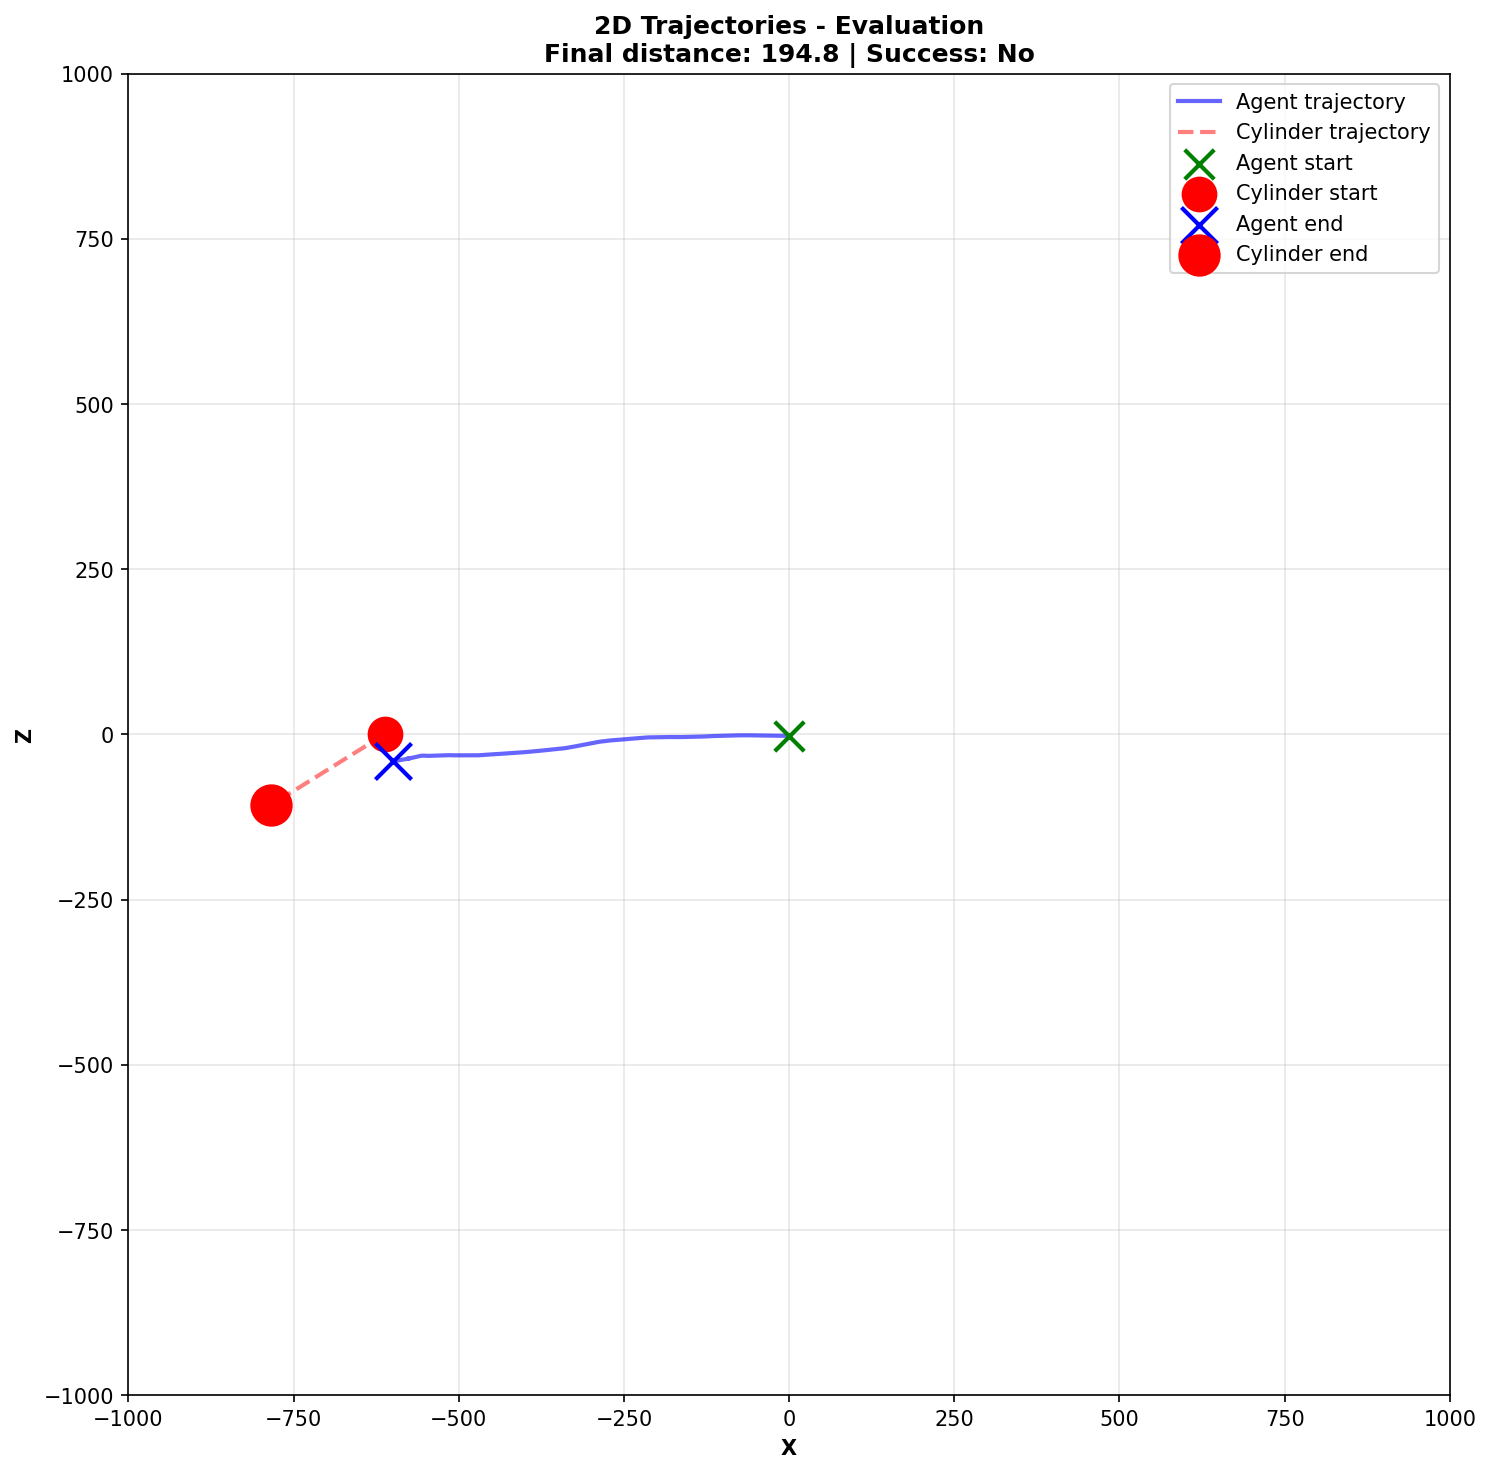
\includegraphics[width=0.7\textwidth]{evaluation_trajectory.png}
    \caption{Trayectoria del agente (azul) siguiendo el cilindro móvil (rojo). Los puntos coloreados indican la progresión temporal.}
    \label{fig:trajectories}
\end{figure}

\subsection{Rendimiento del Sistema}

\begin{table}[H]
\centering
\begin{tabular}{@{}lc@{}}
\toprule
\textbf{Métrica} & \textbf{Valor} \\ \midrule
Pasos para convergencia & $\sim$300 \\
Tasa de éxito (d < 150) & XX\% \\
Distancia final promedio & XXX unidades \\
Recompensa media final & X.XX \\
Tiempo de entrenamiento & XX min \\ \bottomrule
\end{tabular}
\caption{Métricas de rendimiento del sistema}
\end{table}

\section{Conclusiones}

\subsection{Logros}
\begin{itemize}
    \item Implementación exitosa de un entorno Gymnasium personalizado
    \item Entrenamiento efectivo con SAC en espacio continuo
    \item El agente aprende a seguir objetivos móviles
    \item Función de recompensa multi-componente efectiva
\end{itemize}

\subsection{Limitaciones y Trabajo Futuro}
\begin{itemize}
    \item \textbf{Timesteps limitados}: Solo 400 pasos, más entrenamiento mejoraría el rendimiento
    \item \textbf{Generalización}: Evaluar con diferentes velocidades del objetivo
    \item \textbf{Obstáculos}: Extender a entornos con obstáculos
    \item \textbf{Robot real}: Validar en hardware físico
\end{itemize}

\subsection{Lecciones Aprendidas}
\begin{enumerate}
    \item La normalización de observaciones es crucial para el aprendizaje
    \item El balance de componentes en la función de recompensa requiere ajuste fino
    \item SAC es efectivo para control continuo pero requiere suficientes datos
    \item La información visual complementa bien los datos de posicionamiento
\end{enumerate}

\section{Instrucciones de Ejecución}

\subsection{Dependencias}
\begin{lstlisting}[language=bash]
pip install gymnasium stable-baselines3 
pip install numpy pandas matplotlib seaborn
pip install robobopy robobosim
\end{lstlisting}

\subsection{Entrenamiento}
\begin{lstlisting}[language=bash]
python train.py
\end{lstlisting}

\subsection{Evaluación}
\begin{lstlisting}[language=bash]
python eval.py
\end{lstlisting}

\end{document}
